\documentclass[12pt,a4paper]{article}

\usepackage{composites2019}

%% Numbered
%\bibliographystyle{model1-num-names}

%% Numbered without titles
%\bibliographystyle{model1a-num-names}

%% Harvard
%\bibliographystyle{model2-names.bst}\biboptions{authoryear}

%% Vancouver numbered
%\usepackage{numcompress}\bibliographystyle{model3-num-names}

%% Vancouver name/year
%\usepackage{numcompress}\bibliographystyle{model4-names}\biboptions{authoryear}

%% APA style
%\bibliographystyle{model5-names}\biboptions{authoryear}

%% AMA style
%\usepackage{numcompress}\bibliographystyle{model6-num-names}

%% `Elsevier LaTeX' style
%\bibliographystyle{elsarticle-num}
%%%%%%%%%%%%%%%%%%%%%%%

\begin{document}
\thispagestyle{empty}

\vspace*{-3.4cm}
\begin{table}[!h]
\begin{tabular}{r}
\hspace*{2.9cm} \scriptsize \textsf{7th ECCOMAS Thematic Conference on the Mechanical Response of Composites: COMPOSITES 2019} \\
\hspace*{2.9cm} \tiny \textsf{A. Turon, P. Maimí \& M. Fagerström (Editors)}
\end{tabular}
\end{table}

\vspace*{-0.7cm}

\begin{center}
\title{ESTIMATING THE SIZE DISTRIBUTION OF THE FIBER/MATRIX INTERFACE CRACK IN MICROSTRUCTURAL MODELS OF UD AND CROSS-PLY LAMINATES BY A LINEAR ELASTIC FRACTURE MECHANICS APPROACH}
\end{center}
\begin{center}
\textbf{\underline{Luca Di Stasio}$^{1,2,*}$, Janis Varna$^{2}$, Zoubir Ayadi$^{1}$} \\ [7pt]
\small{$^1$~Universit\'e de Lorraine, EEIGM, IJL, 6 Rue Bastien Lepage, F-54010 Nancy, France}  \\  [2pt]
\small{$^2$~Lule\aa\ University of Technology, University Campus, SE-97187 Lule\aa, Sweden}  \\  [2pt]
\small{$^*$~\texttt{luca.di.stasio@ltu.se}} \\
\end{center}

\noindent
The recent interest in \emph{thin-ply} laminates for advanced applications~\cite{Kopp2017} has led to a renewed focus on transverse cracks onset. Tranverse cracking manifests itself at first in the form of fiber/matrix interface cracks (debonds), that propagate along the arc direction of the fiber surface and coalesce together to form a continouos through-the-thickness crack. Characterization of this process has been mainly directed to the evaluation of the Energy Release Rate (ERR); however, the attention has been devoted to the study of a central partially debonded fiber placed in an effectively medium and the effect of nearby fibers~\cite{Sandino2016}. In this work, the ERR in Mode I and Mode II is evaluated for debonds appearing in Representative Volume Elements (RVEs) of regular microstructures of UD and cross-ply laminates. We then consider a mixed-mode criterion for propagation and analyze the effect of the size of the initial flaw and of the mode sensitivity parameter, thus leading to the estimation of the expected size distribution of a debond in these representative microstructures. Finally, the results are compared with available microscopic observations~\cite{Correa2018}.

\begin{figure}[h]
\centering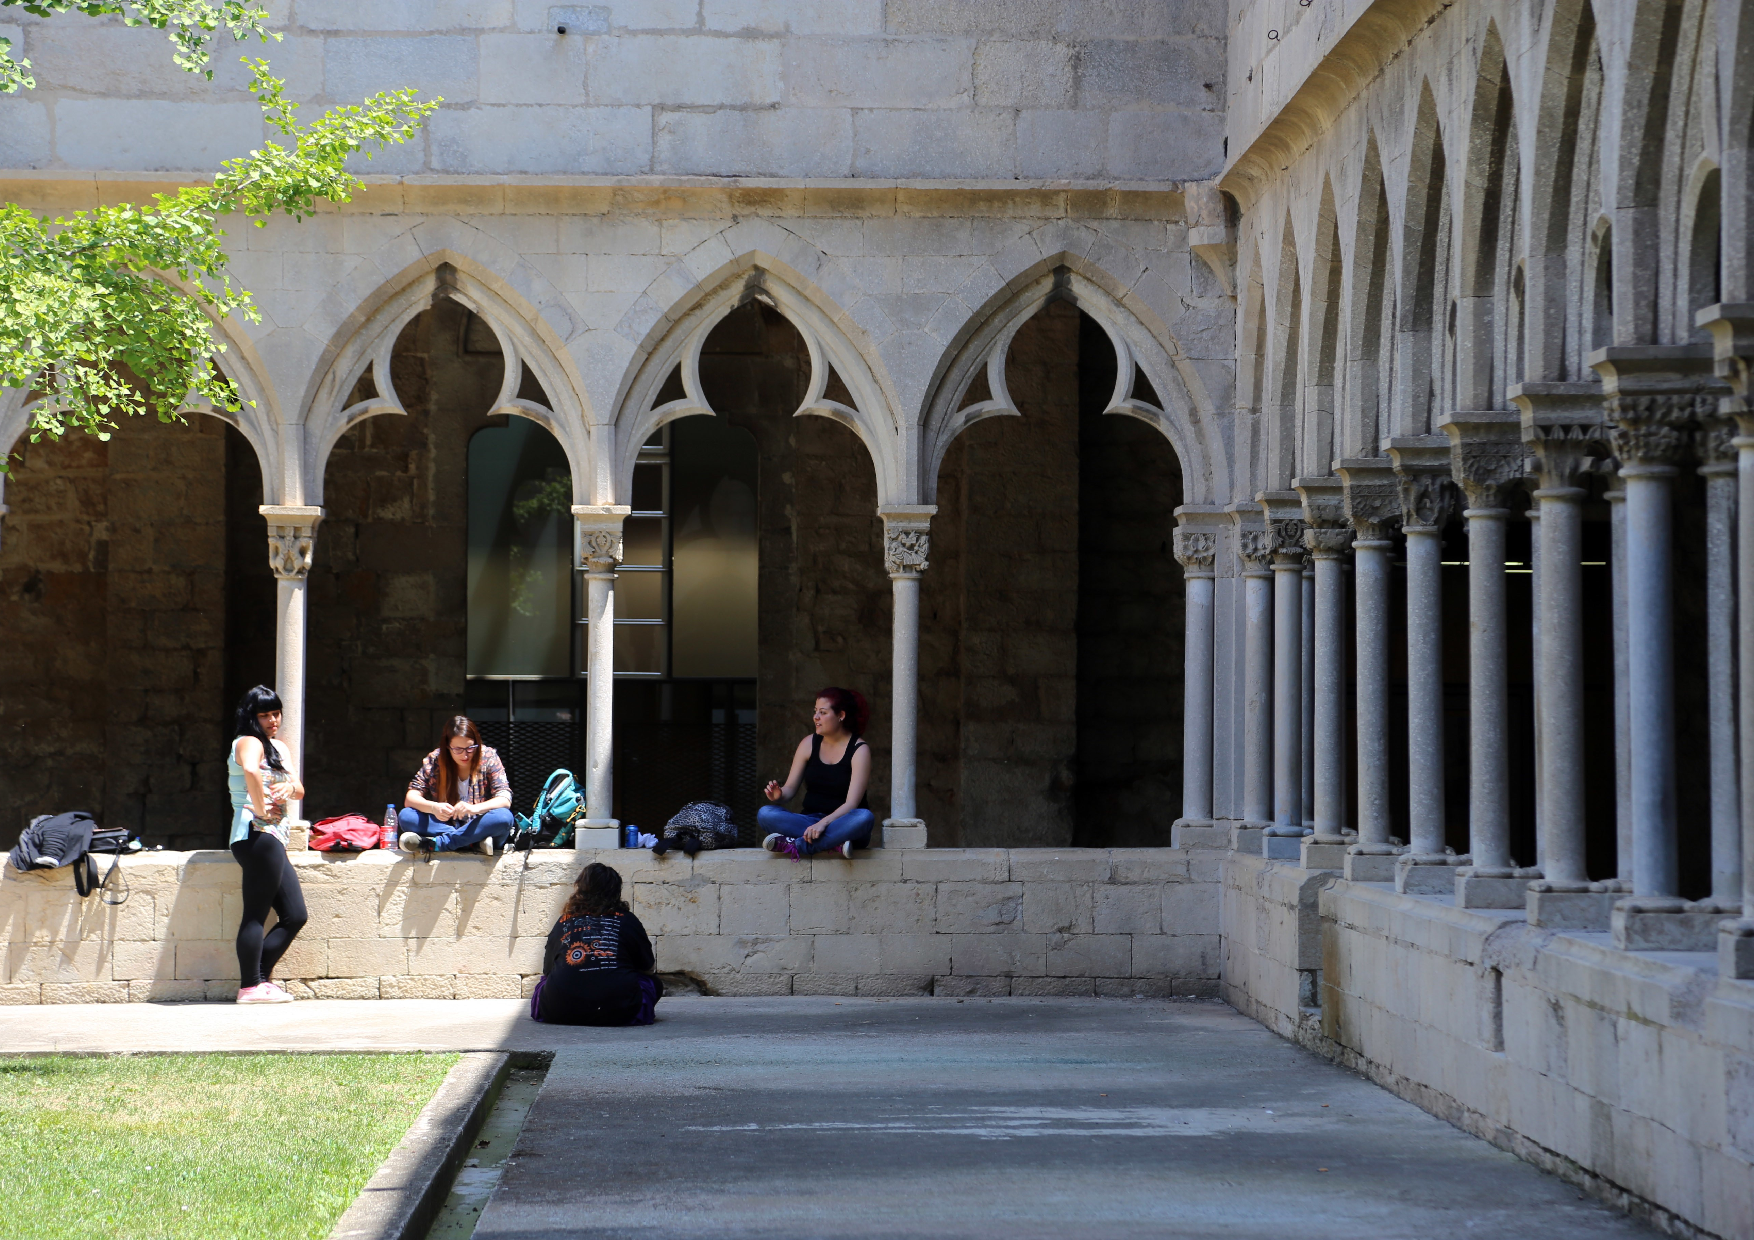
\includegraphics[width=0.55\linewidth]{Claustre.pdf}
\caption{The former cloister of the convent of St. Domènec, which is the venue of this conference.}
\label{fig:Claustre}
\end{figure}

\begin{thebibliography}{9}
%
%% === Replace this by your references ===
%
\bibitem{Kopp2017} A. Kopp, S. Stappert, D. Mattsson, K. Olofsson, E. Marklund, G. Kurth, E. Mooij and Evelyne Roorda (2017) The Aurora space launcher concept. \textit{CEAS Space Journal}, \textbf{10}, 167--187.
\bibitem{Sandino2016} C. Sandino, E. Correa and F. Par{\'{\i}}s (2016) Numerical analysis of the influence of a nearby fibre on the interface crack growth in composites under transverse tensile load. \textit{Engineering Fracture Mechanics}, \textbf{168}, 58--75.
\bibitem{Correa2018} E. Correa, M. I. Valverde, M .L. Velasco and F. París (2018) Microscopical observations of inter-fibre failure under tension. \textit{Engineering Fracture Mechanics}, \textbf{155}, 213--220.
%\bibitem{Pimenta} S. Pimenta and S.T. Pinho (2012) The effect of recycling on the mechanical response of carbon fibres and their composites. \textit{Composite Structures}, \textbf{94}, 3669-3684.
%
\end{thebibliography}

\end{document}
  
